% Preliminary Study about Design Patterns Selection

%Chapter introduction
% Ligação com o que veio antes
% Objetivo do capítulo no contexto da tese
% Conteúdo do capítulo

The previous chapter explored the evolution of AI, particularly in large language models and prompt engineering, and trends in software design patterns. Now, we focus on the practical application of these concepts. This chapter is a crucial bridge between the Literature Review and applied methodologies the aims to conduct an empirical study on selecting design patterns in software architecture. The study aims to identify areas where AI, particularly prompt engineering, could enhance the decision-making process in software design.

\textbf{Study Description:}Introduces the methodology, scope, and study participants. This sets the stage for understanding the findings' context and relevance.\textbf{Research Questions for Design Pattern Selection:}Presents the specific questions this study aims to address, linking to the gaps identified in the Literature Review.\textbf{Questions Collection:}Describes the process of gathering relevant questions and criteria used in the design pattern selection process, providing insights into the practical considerations of software architects.\textbf{Design Patterns Selection Results:}Analyzes the results obtained from the study, offering a comprehensive view of the current state of design pattern selection practices.\textbf{Discussion of the Findings:}Discuss the implications of the study’s findings, particularly in integrating AI tools for decision-making in software architecture.

\section{Study description}

General-purpose AI-assisted tools, such as ChatGPT, have recently gained much attention from the media and the general public. That raised questions about in which tasks we can apply such a tool. A code design is essential for agile software development to keep it ready for change. 

In this context, identifying which design pattern can be appropriate for a given scenario can be considered an advanced skill that requires a high degree of abstraction and a good knowledge of object orientation. This preliminary study with design pattern questions aimed to perform an exploratory study investigating the effectiveness of an AI-assisted tool in assisting developers in choosing a design pattern to solve design scenarios. To reach this goal, we gathered 56 existing questions used by teachers and public tenders that provide a concrete context and ask which design pattern would be suitable. 

We submitted these questions to ChatGPT and analyzed the answers. We found that 93\% of the questions were answered correctly with a good level of detail, demonstrating the potential of such a tool as a valuable resource to help developers apply design patterns and make design decisions.

% ---------------------------------------------------------------------------
% Inicio da introdução
% ---------------------------------------------------------------------------
%\section{Contextualization of the preliminary study}\label{ContextPreliminaryStudy}


% ***************************************************************************
% Fim da Introdução
% ***************************************************************************

% ---------------------------------------------------------------------------
% Inicio da Seção Research Methodology
% ---------------------------------------------------------------------------

\section{Research Questions Design Pattern Selection}\label{ResearchPreliminaryStudy}

Based on the goal of investigating if an AI-assisted tool can help developers in choosing the appropriate design pattern to apply in a given scenario, we formulated three more specific research questions for this preliminary study of automatic design patterns selection:

\begin{itemize}
    \item \textbf{\textit{RQPS\textsubscript{1}}} - How is the success rate of the AI-assisted tool in suggesting design patterns?
    \item \textbf{\textit{RQPS\textsubscript{2}}} - Do elements provided in the answer of the AI-assisted tool help in the pattern implementation?
    \item \textbf{\textit{RQPS\textsubscript{3}}} - In questions where the wrong pattern is pointed, does the AI-assisted tool answer mislead the developers?
\end{itemize}

To answer these research questions, we collected preexisting questions prepared by higher education professors or public tenders in which a scenario is described, and it asks which design pattern should be applied. Since these questions are used to evaluate the student's knowledge of patterns, we believe they can also be used to evaluate the tool's performance. We chose ChatGPT as the AI-assisted tool for the study and submitted the selected questions to it, registering the answers. The content of the answers was analyzed, not only comparing to the exercise correct answer \textbf{\textit{RQPS\textsubscript{1}}} but also analyzing what elements that can help the developers in the pattern implementation were present \textbf{\textit{RQPS\textsubscript{2}}}. A qualitative analysis was done on the wrong answers to evaluate if they could mislead the developers \textbf{\textit{RQPS\textsubscript{3}}}.

To select the answers, we contacted professors that teach design patterns in universities asking for exam questions and exercises they give students. We've received the material from three professors from different countries: Italy, the United States, and Portugal. We also analyzed available exams of public tenders for 26 Brazilian institutions. As a question inclusion criteria for this study, we considered the following criteria: 


\begin{enumerate}
    \item The solution should be one of the “Gang of Four” (GoF) patterns; 
    \item The question should describe a scenario and ask which pattern should be applied;
    \item The question should describe a concrete scenario and not just give general requirements. 
\end{enumerate}


The first criterion was included to restrict the scope of the study to these patterns, which are well known by the software development community and taught in university courses, which enabled finding a good number of questions. The two other criteria were considered to choose questions that better simulate the decision of applying a pattern in a real scenario.

The qualitative analysis inspected each correct answer and evaluated the following criteria of the preliminary study of automatic design patterns selection(CPS): 
\begin{itemize}
\item \textbf{\textit{CPS\textsubscript{1}}} - If the answer mentions the described context (instead of just giving a generic answer); 
\item \textbf{\textit{CPS\textsubscript{2}}} - If the answer explains the pattern;
\item \textbf{\textit{CPS\textsubscript{3}}} - If the answer describes the classes and interfaces that need to be created to implement the pattern; 
\item \textbf{\textit{CPS\textsubscript{4}}} - If the answer describes the methods that should be created to implement the pattern; 
\item \textbf{\textit{CPS\textsubscript{5}}} - If the answers included a UML diagram to represent the solution; 
\item \textbf{\textit{CPS\textsubscript{6}}} - If the answer described any trade-off or negative consequence in using of the proposed pattern.
\end{itemize}

\section{Questions Collection}\label{QuestionDatabasePreliminaryStudy}

In selecting questions, we obtained a total of 56 Design Pattern questions. There are 19 questions from university courses: 9 questions from the United States, 6 from Portugal, and 4 from Italy. We also found 37 questions in Portuguese from public tenders in Brazil, inspecting selection exams of twenty-nine different institutions shown in Table~\ref{table:instituttion}. Since the questions obtained from teachers are used in exams and some asked to keep them private, we did not make the questions dataset open.

\begin{table}[!ht]
    \small
    \centering
    \caption{Number of questions by institutions, countries, and language}
    \label{table:instituttion}
    \begin{tabular}{llll}
        \toprule
        \hline
        \rowcolor{gray!19} \textbf{Institution} & \textbf{Country} & \textbf{Portuguese} & \textbf{English} \\ \hline
        Banco Nacional de Desenvolvimento Econômico & Brazil & 1 & ~ \\
        \rowcolor{gray!19} Caixa Economica Federal & Brazil & 1 & ~ \\ 
        Companhia Catarinense de Água e Saneamento & Brazil & 1 & ~ \\
        \rowcolor{gray!19} Companhia do Metropolitano de São Paulo & Brazil & 1 & ~ \\ 
        Companhia Docas do Estado da Bahia & Brazil & 1 & ~ \\ 
        \rowcolor{gray!19} Companhia Hidro Elétrica do São Francisco & Brazil & 1 & ~ \\ 
        Defensoria Pública de São Paulo & Brazil & 1 & ~ \\ 
        \rowcolor{gray!19} Defensoria Pública do Estado do Rio de Janeiro & Brazil & 2 & ~ \\ 
        Defensoria Pública do Rio Grande do Sul & Brazil & 1 & ~ \\ 
        \rowcolor{gray!19} Instituto Brasileiro de Geografia e Estatística & Brazil & 4 & ~ \\ 
        Ministério Público do Estado da Paraíba & Brazil & 1 & ~ \\ 
        \rowcolor{gray!19} Ministério Público do Estado de Alagoas & Brazil & 1 & ~ \\ 
        Petrobras Distribuidora S.A. & Brazil & 1 & ~ \\ 
        \rowcolor{gray!19} Petrobras Transporte S.A. & Brazil & 5 & ~ \\ 
        Petróleo Brasileiro S.A. & Brazil & 4 & ~ \\ 
        \rowcolor{gray!19} Reguladora de Serviços Públicos Delegados de SP & Brazil & 1 & ~ \\ 
        Saneamento de Goiás S.A. & Brazil & 1 & ~ \\ 
        \rowcolor{gray!19} Tribunal de Contas do Estado de Rondônia & Brazil & 1 & ~ \\ 
        Tribunal Regional Eleitoral da Paraíba & Brazil & 1 & ~ \\ 
        \rowcolor{gray!19} Tribunal Regional Eleitoral da São Paulo & Brazil & 1 & ~ \\ 
        Tribunal Regional Federal da 4ª Região & Brazil & 1 & ~ \\ 
        \rowcolor{gray!19} Tribunal de Contas do Estado de Alagoas & Brazil & 1 & ~ \\ 
        Universidade do Estado do Amapá & Brazil & 1 & ~ \\ 
        \rowcolor{gray!19} Universidade Federal de Alagoas & Brazil & 1 & ~ \\ 
        Universidade Federal do Ceará & Brazil & 1 & ~ \\ 
        \rowcolor{gray!19} Vestibular da Universidade Estadual Paulista & Brazil & 1 & ~ \\ 
        Free University of Bozen-Bolzano & Italy & ~ & 4 \\
        \rowcolor{gray!19} Faculdade de Engenharia da Universidade do Porto & Portugal & ~ & 6 ~ \\ 
        University Northern Arizona & USA & ~ & 9 ~\\ \hline
         \bottomrule
    \end{tabular}
    \objectsource{\objectsourceauthor}
\end{table}

From the selected questions, all patterns in the study scope were covered with at least one question. Figure~\ref{number-questions} presents how many questions have each pattern as a correct answer.
  
\begin{figure}[!ht]
\centering
\caption{\centering Number of questions collected by design patterns.}\label{number-questions}
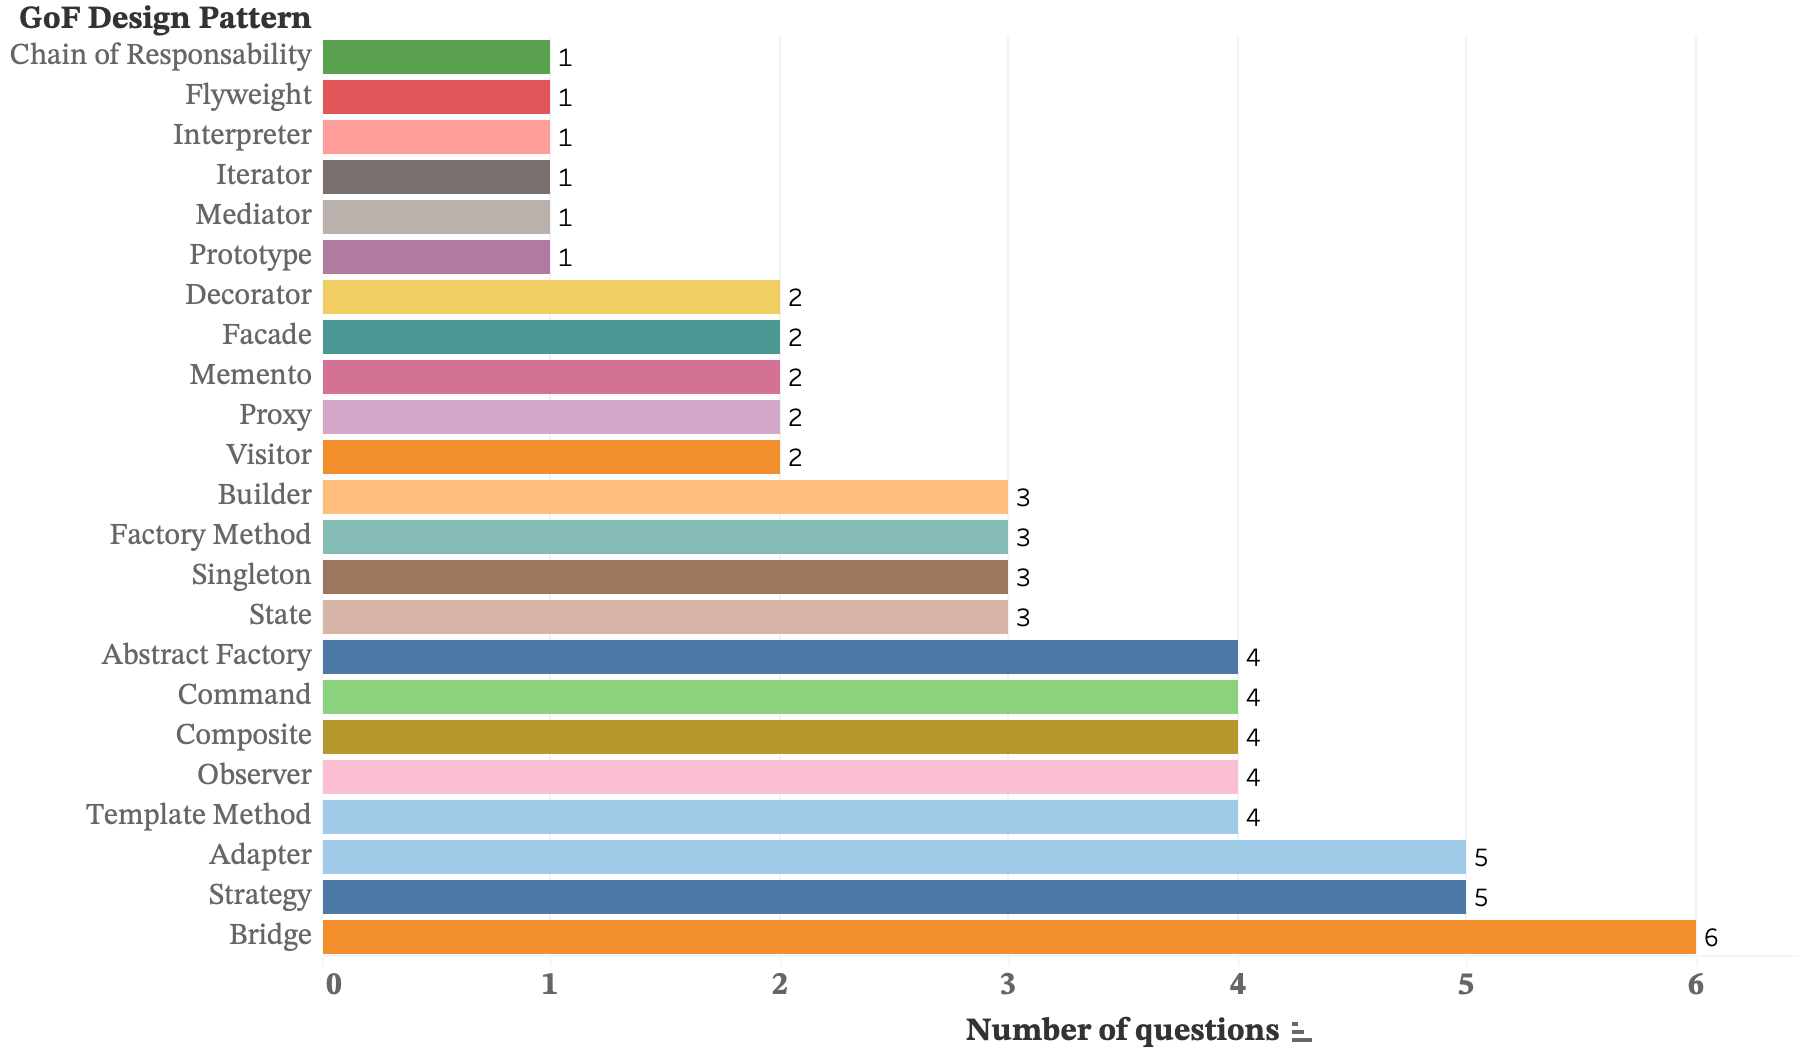
\includegraphics[width=0.7\textwidth]{figures/number-questions.png}
 \objectsource{\objectsourceauthor}
\end{figure}

Considering the pattern categories Figure~\ref{type-patterns}, there are 25 questions about \textit{behavioral} pattern, 22 about \textit{structural} patterns, and 17 about \textit{creational} patterns. We consider that the question database is reasonably balanced among the pattern categories Figure~\ref{type-patterns}, having a good amount of questions that cover each one. Two questions accepted more than one pattern as a correct answer; in such cases, we consider any one of them as right. Four questions asked for a combination of patterns as an answer; in this case, we considered that the right answer should include all of them.

\begin{figure}[!ht]
\centering
\caption{\centering Number of questions collected per design pattern category.}\label{type-patterns}
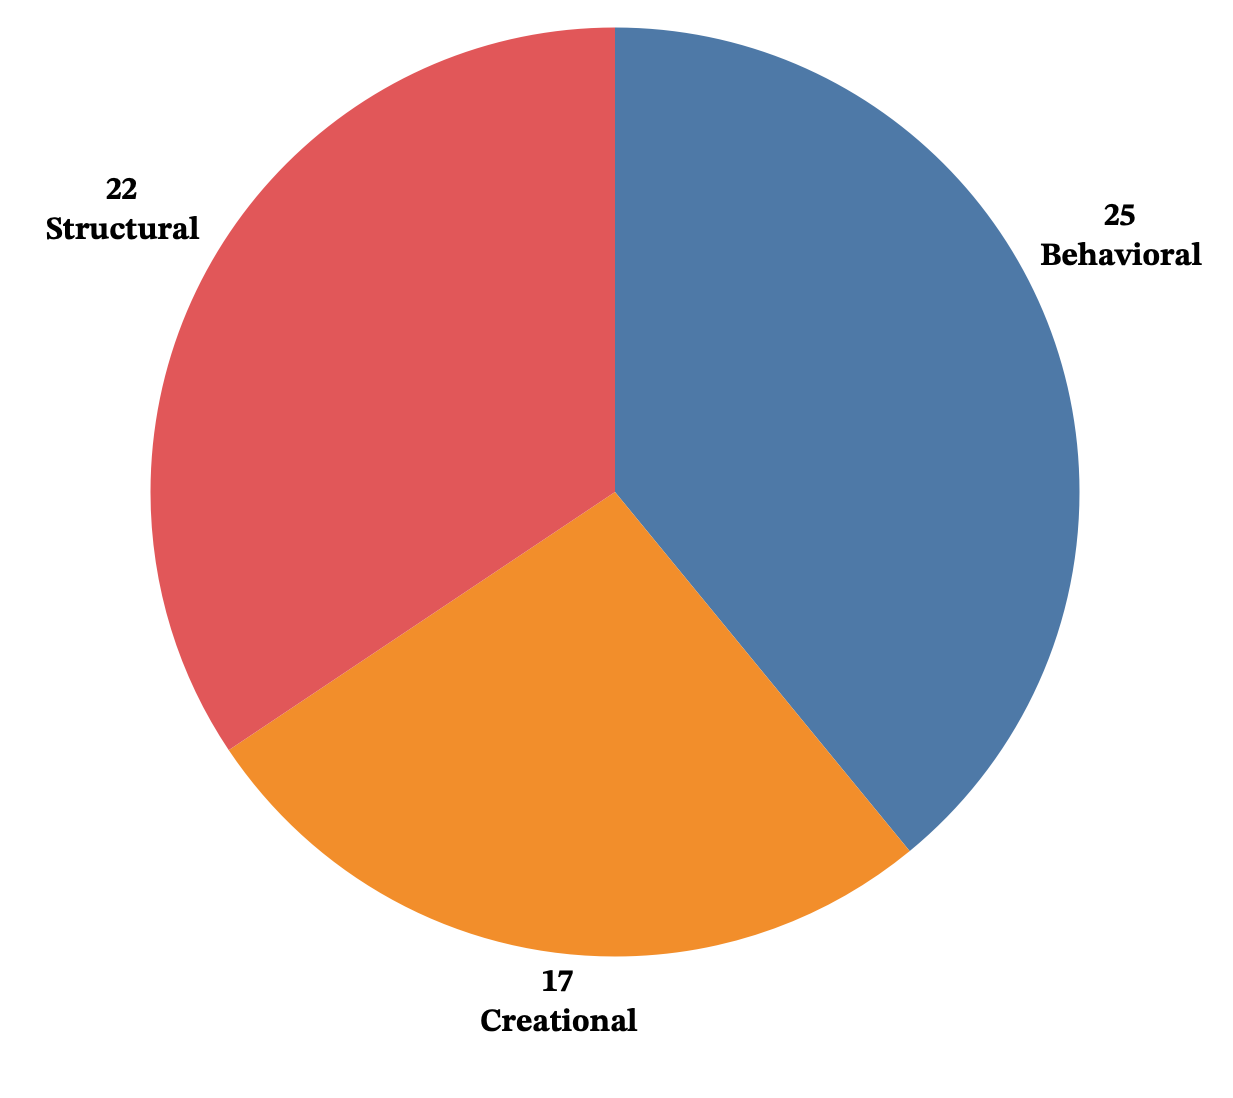
\includegraphics[width=0.6\textwidth]{figures/types-patterns.png}
 \objectsource{\objectsourceauthor}
\end{figure}

% ---------------------------------------------------------------------------
% Inicio da Seção Results
% ---------------------------------------------------------------------------
\section{Results}\label{ResulttsPreliminaryStudy}

The questions were sent to ChatGPT (version 3.5) in the period comprised between 2023-03-03 and 2023-04-16. Based on the results, ChatGPT was generally effective in answering our questions, with an overall accuracy rate of 93\%. Most of the questions were in Portuguese, with 31 of the 34 questions answered correctly, while 21 of the 22 in English were answered correctly. 

The answers have an average number of 1033 chars with a standard deviation of 657, varying from a minimum of 247 to a maximum of 3127. Considering the number of words, the average is 155, with a standard deviation of 89, varying from a minimum of 37 to a maximum of 390 words. We used the Pearson correlation coefficient to evaluate if the number of words on the question would be related to the number of words in the answer; more details in Figure~\ref{avg-words-patterns}. The value of 0,09 obtained showed that there was no significant relation. 

\begin{figure}[!ht]
\centering
\caption{\centering Average words per design pattern.}
\label{avg-words-patterns}
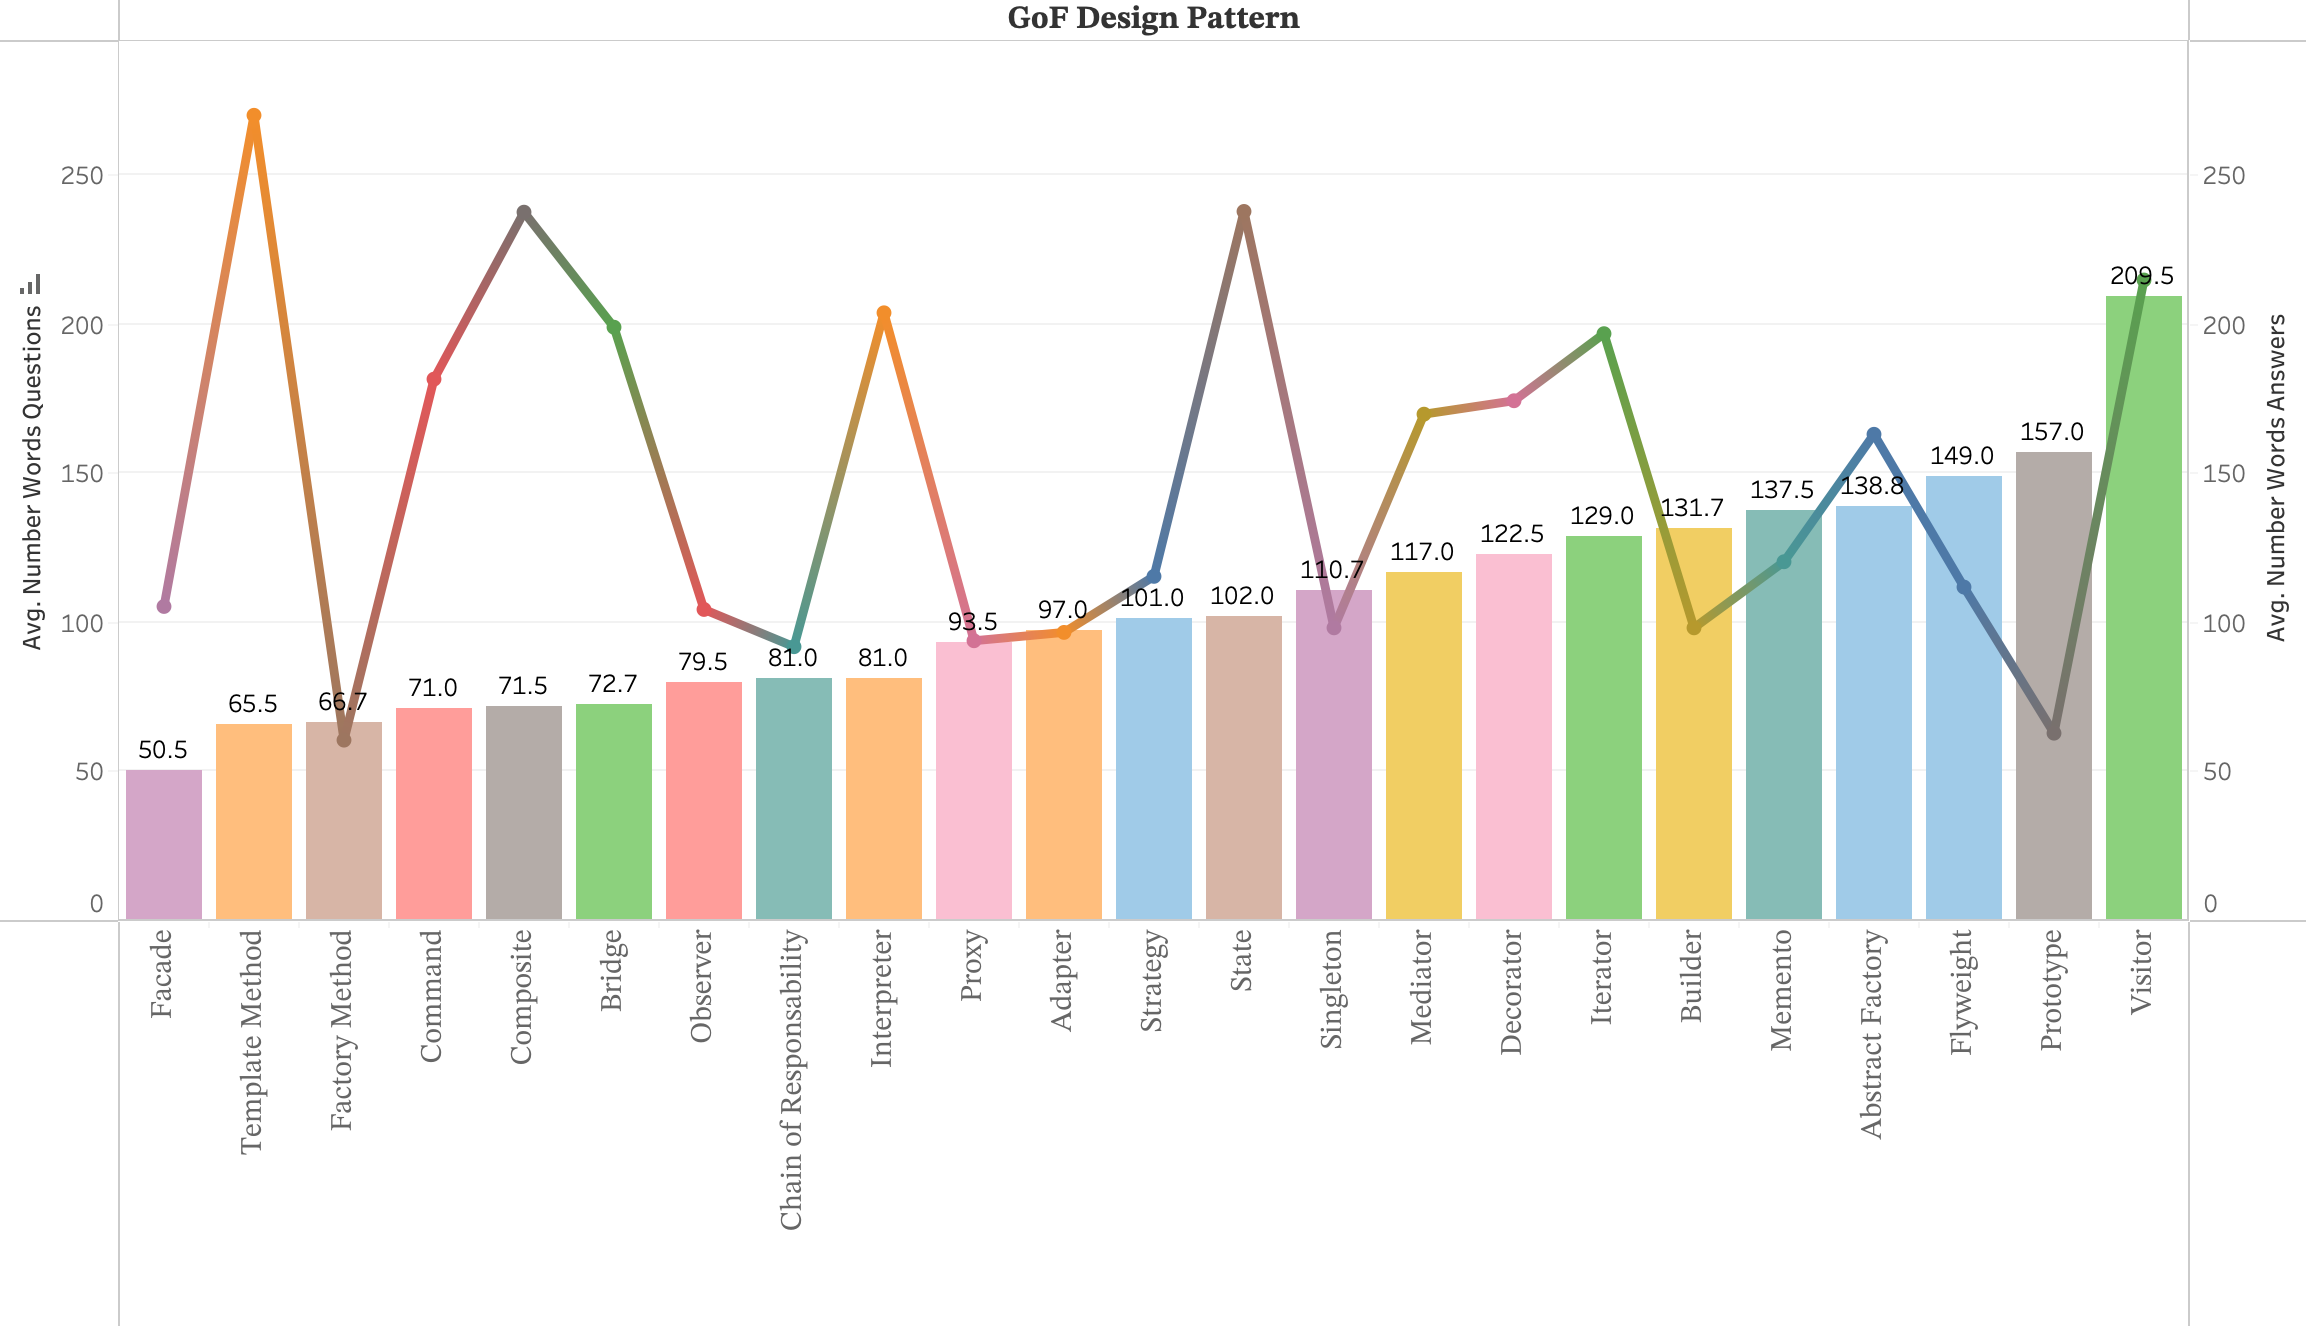
\includegraphics[width=0.9\textwidth]{figures/questions-patterns-avg-words.png}
 \objectsource{\objectsourceauthor}
\end{figure}

\textbf{Information Present in the Answers.} A qualitative analysis evaluated the six criteria proposed in Section~\ref{ResearchPreliminaryStudy}. In Table~\ref{table:cps} are the results:

\begin{table}[!ht] 
    \small
    \centering
    \caption{(CPS: Criteria Number),(Rate: Percentage of correct answers for each criterion), (A/Q: Number of correct answers versus total questions), and Criteria Description.}
    \label{table:cps}
    \begin{tabular}{p{0.4in}p{0.5in}p{0.5in}p{4.0in}}       
        \toprule
         \hline
        \rowcolor{gray!19} \textbf{CPS}  & \textbf{Rate} & \textbf{A/Q} & \textbf{Criteria Description}  ~\\ \hline
        % \midrule
        \textbf{\textit{CPS\textsubscript{1}}} & 100\% & 52/52 & Mention the described context instead of just giving a generic answer. ~\\ \hline
        \rowcolor{gray!19} \textbf{\textit{CPS\textsubscript{2}}} & 57.69\% & 30/52 & Explained the Design pattern of the question elaborated.  ~\\ \hline
       \textbf{\textit{CPS\textsubscript{3}}} & 32.69\% & 17/52  & Describe the classes and interfaces that need to be created to implement the pattern. ~\\ \hline
       \rowcolor{gray!19} \textbf{\textit{CPS\textsubscript{4}}} & 26.92\% & 14/52  & Describe the methods that should be created to implement the pattern. ~\\ \hline
       \textbf{\textit{CPS\textsubscript{5}}} & 3.85\% & 2/52  & Include a UML diagram to represent
        the solution. ~\\ \hline
       \rowcolor{gray!19} \textbf{\textit{CPS\textsubscript{6}}} & 0\% & 0/52  & Describe any trade-off or negative consequence in using the proposed pattern. ~\\ \hline
       \bottomrule
    \end{tabular}
    \objectsource{\objectsourceauthor}
\end{table}


\textbf{Assessment of Wrong Answers.} This section presents an analysis of the questions that received a wrong answer (the ID will be used to refer to that question later):

\begin{itemize}
    \item  \textbf{\textit{WA\textsubscript{1}}} - The question presented a problem in creating a solution for reports needing two dimensions: the report type and the report format. While the correct answer was using the Visitor pattern, the tool suggested Strategy. In the answer, one of the dimensions of the question was ignored, and the proposed solution focused only on the report format.
    \item \textbf{\textit{WA\textsubscript{2}}} - The question asked how the representation of more complex devices could be dynamically created by reusing the behavior of more simple devices that are part of it. While the correct answer was Composite, the given answer was Factory Method. In this case, the solution described does not help in solving the design problem presented.
    \item \textbf{\textit{WA\textsubscript{3}}} - The question presented the context of exchanging messages between different cell phone operating systems platforms, handling distinct message formats transparently. While the correct answer was Adapter, the answer given was Bridge. In this case, even if the patterns share some structural similarities, the described solution does not help solve the problem.
    \item \textbf{\textit{WA\textsubscript{4}}} - The question presented an abstract class that is responsible for transparently creating objects corresponding to different types of databases. Concrete subclasses are responsible for instantiating specific connections and queries for each type of database. The correct answer was Abstract Factory, and the given answer was Factory Method. Even if both are creational patterns, the given answer does not help to solve the problem because it was necessary to create a family of objects for each type of database.
\end{itemize}

% ---------------------------------------------------------------------------
% Inicio da Seção Discussion
% ---------------------------------------------------------------------------
\section{Discussion}\label{DiscussionPreliminaryStudy}

This section performs a discussion based on the obtained results, answering each research question. We also point out some limitations of the present study.

\begin{itemize}
    \item  \textbf{\textit{RQPS\textsubscript{1}}} - How is the success rate of the AI-assisted tool in suggesting design patterns?\label{sec5sub1}
    
    The study showed an efficient result with 93\% correct answers in 56 questions. We highlight that the questions selected do not just ask for information about the patterns but present a specific and concrete scenario. To correctly answer the question by choosing the right pattern, the relevant factors that point to the usage of that specific pattern need to be identified in the context description. We also highlight that in the four questions that required a combination of patterns as an answer, the correct answer was provided by the AI-assisted tool.

    ChatGPT performance can be considered good compared to other works that proposed more specific techniques for pattern suggestion~\cite{Hussain2019automated, Naghdipour2023Semi}. Consequently, it can be considered a suitable assisting tool for developers, which can describe the design scenario in their application and receive suggestions from the tool.

     \item  \textbf{\textit{RQPS\textsubscript{2}}}  - Do elements provided in the answer of the AI-assisted tool help in the pattern implementation?\label{sec5sub2}

     One positive point is that all responses mentioned the problem's context instead of just pointing to the pattern and providing a generic explanation. Around one-third of the answers also provided the name of the classes and interfaces that should be created in that case. Additionally, around one-quarter described the methods that should be created. Few answers, only 2, also provided UML diagrams with the structure that should be used.

    Most of the answers, but not all, brought a more theoretical explanation of the pattern, which can be useful in case the developer is unfamiliar with the pattern. A piece of important information that was not present in any of the answers is the trade-off in the usage of the suggested pattern since knowing possible bad consequences is important to make design decisions.
    
    To avoid any kind of bias, the questions used in this study were not modified; however, we acknowledge that if we explicitly included in the question what information we wanted in the answer, the tool would include it. We did some exploratory experiments on some of the questions, rephrasing them to ask explicitly for some missing information. As a result, the missing information was included correctly in the new answers. That fact highlights the importance of how the questions are formulated, a new disciple called prompt engineering~\cite{White2023}.  

    \item  \textbf{\textit{RQPS\textsubscript{3}}} - In questions where the wrong pattern is pointed, does the AI-assisted tool answer mislead the developers?\label{sec5sub3}

    We analyzed the four questions that received wrong answers to see if there was any inconsistency or ambiguity in the way they were formulated, and all authors agreed that they were clearly described and there was no doubt about the correct answer. For all the patterns that were the correct answer for these questions, there is at least another question with the same pattern answered correctly.

    In the case of \textbf{\textit{WA\textsubscript{1}}}, the answer given by ChatGPT considered the described context partially, and the Strategy implementation that it described could be evolved to a Visitor. However, in \textbf{\textit{WA\textsubscript{2}}}, \textbf{\textit{WA\textsubscript{3}}}, and \textbf{\textit{WA\textsubscript{4}}}, the answer leads to a way that does not solve the problem. The answers are assertive and well-described, and we believe can easily be accepted by a less experienced developer. Because of that, we advise that the answers given by an AI-assisted tool should be reviewed and understood instead of being blinded implemented. In other words, there should be a professional that should be responsible for its analysis and adoption.
    
    We also noticed that some of these questions used terms and expressions closely connected to other patterns. So, we suggest avoiding expressions like "family of algorithms" or "composite objects" that can drive the tool to a specific pattern.
    
\end{itemize}

\MyPara{Limitations of Design Patterns Selection}\label{sec5sub4}

Our study focused only on "Gang of Four" (GoF) design patterns, which are well-known and widely used in the software development community. The performance of ChatGPT may differ for other design patterns that are newer and have less material available.

Our study was conducted in a controlled setting using preexisting questions. These questions were formulated by teachers with software design knowledge, focused on scenarios suitable for applying one of the patterns, and included all the necessary information relevant to direct the answer to one of the patterns. Using such a tool in a real project would require skills to identify the relevant forces in the scenario and formulate them properly~\cite{White2023}. Asking which pattern should be used might force the choice of one pattern in cases where none of them is suitable.

% ***************************************************************************
% Fim da Seção Discussion
% ***************************************************************************

% ---------------------------------------------------------------------------
% Inicio da Seção Conclusion
% ---------------------------------------------------------------------------


% ***************************************************************************
% Fim da Seção Conclusion
% ***************************************************************************